%__________________________________________________________________________________________________
\chapter{Scope} 
 
    \section{Introduction}

In this section we take a deeper look at how the scope is treated in Fortran and Python since each programming language has its own particularities. 

Fortran has two units of program (\texttt{program} and \texttt{module}) and two units of subprogram (\texttt{subroutine} and \texttt{function}).
Program units can contain subprograms but remember that some subroutines can also contain functions, and even functions can contain other functions. 
By default, each variable, named constant, object, function or procedure is treated in the following way (see Figure \ref{fig:ScopeFor}):
\begin{itemize}
    \item Everything declared at the beginning of a program/subprogram will be treated as global for that unit. Hence, all units of program nested will see the entity.
    This also includes the \texttt{use} statement, e.g. a main program using a module sees all the global entities of the module (variables, procedures, etc.). 
    
    \item On the contrary, all entities declared inside subroutines and functions are local and its scope is limited to the procedure itself. 
    %Notice that the scope of the procedures follow the same rule, in the figure \ref{fig:ScopeFor} the function \texttt{f2( x )} is only accessible inside the subroutine \texttt{sub2( x )}.
    
    \item Between program units the entities are not shared unless the \texttt{use} statement makes the public entities visible. 
    When we build a module in Fortran we can decide which variables, procedures, etc. are \texttt{public} and which are \texttt{private}. Hence, the main program or a different module that ``uses'' our module only sees the public entities.
    
    \item If a local variable uses the same name as a global variable automatically becomes only local so it won't be able to access or modify the value of the global entity. 
\end{itemize}
 
\begin{figure}[h]
    \centering
    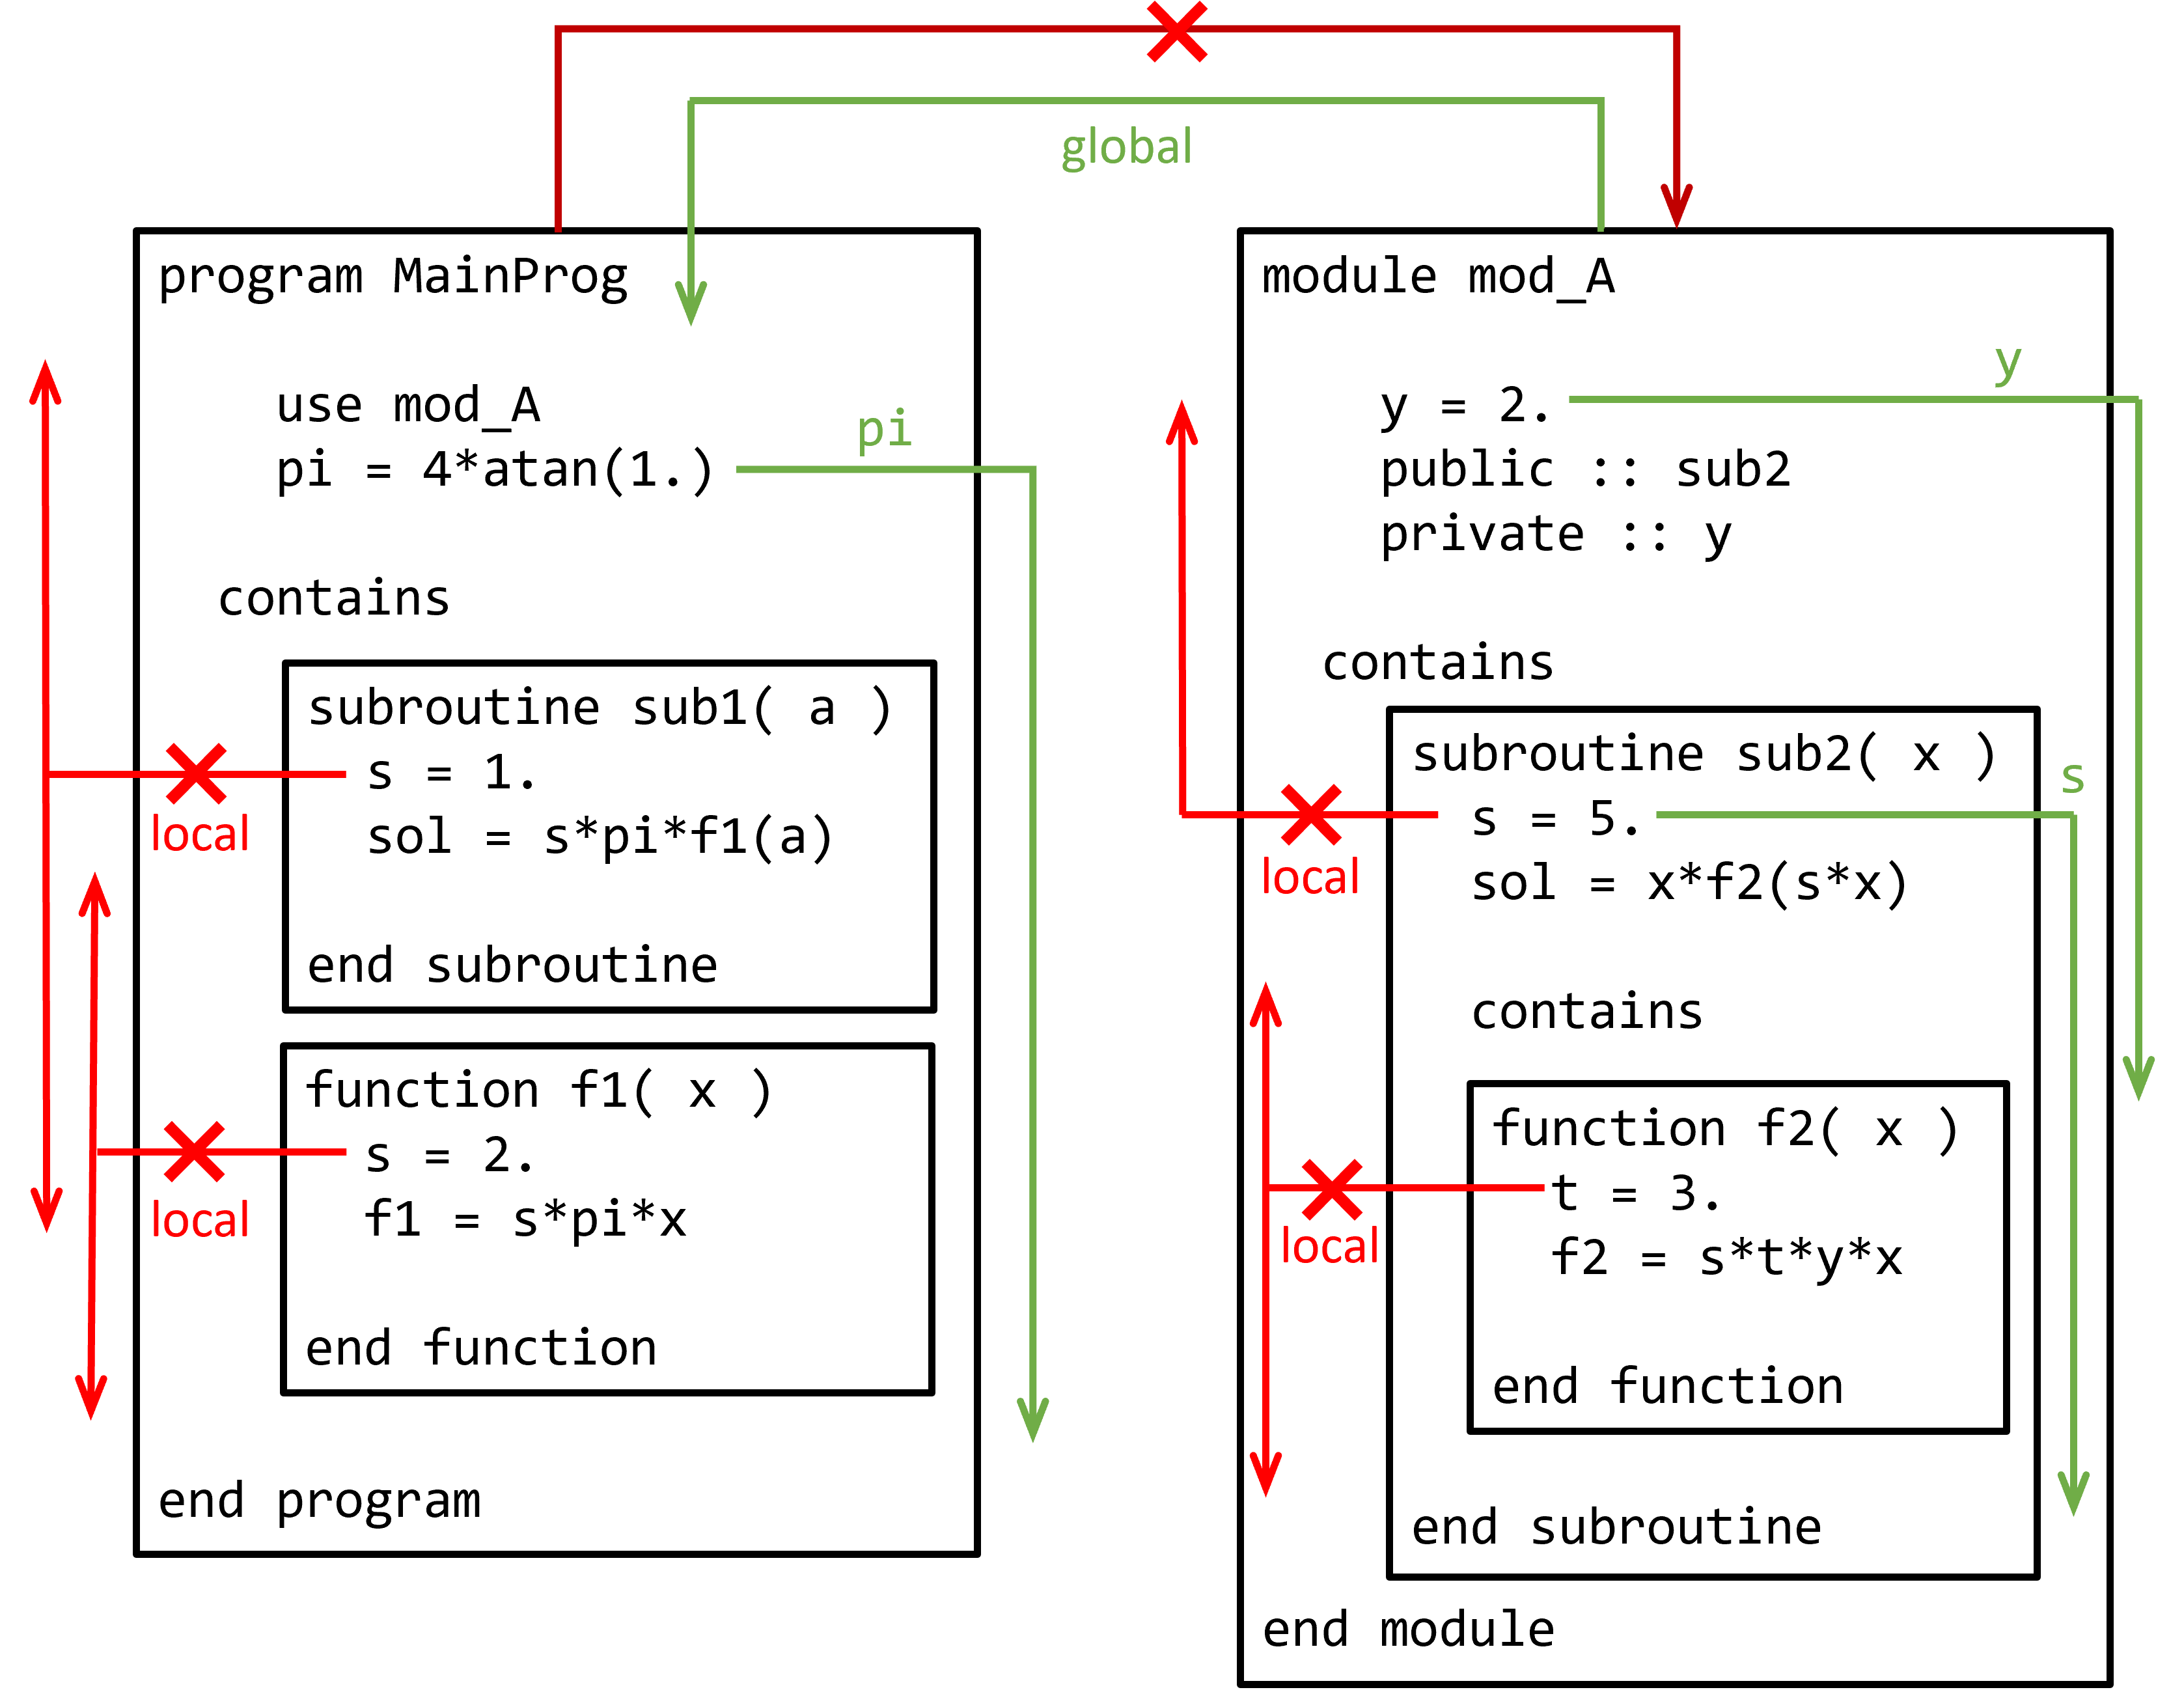
\includegraphics[width= \textwidth]{./doc/Figures/ScopeFor.png}
    \caption{Example of scope for different variables and constants in both program units in Fortran. Notice that \texttt{MainProg} sees all entities of \texttt{mod\_A} by default, however, since \texttt{y} is declared as private, it won't be seen. Furthermore, function \texttt{f2( x )} is only accessible inside the subroutine \texttt{sub2( x )} so it won't be accessible from anywhere else. Finally, notice that \texttt{sub1()} sees \texttt{f1()} since both are global in the main program.}
    \label{fig:ScopeFor}
\end{figure}



%Consejos
%- Cuando usar globales o locales, ciertas normas, declarar todo lo posible como local
%- usar parameter en ciertas globales
%- interfac explicita, en archivos metemos main o modules
%- Datos simepre deben pasarse por cabecera, mencionar


%In the following code,  variables $x, y,z $ are visible inside the subroutine \texttt{Test}.  
In the following code, the variable $y$ is a global variable of module \texttt{modB} and $x$ is a global variable of module \texttt{modA}.  
Then, $y$ is seen inside function \texttt{functionB()} and $x$ is seen in \texttt{functionA}.
All global variables of \texttt{modB} are seen outside by means of the sentence \texttt{use modB}. 
Besides, since \texttt{modB} uses \texttt{modA}, all global variables of \texttt{modA} are seen in \texttt{modB}. 
More specifically, this means that $x$ is also seen in \texttt{functionB()}. 
\vspace{0.5cm} 
 
 
    \newpage  
    \section{Fortran}

\renewcommand{\home}{./Fortran/sources/Advanced_programming/scope} 
\listings{\home/modB.f90}{module modB}{end module}{modB.f90}

\listings{\home/modA.f90}{module modA}{end module}{modA.f90}


    \newpage
    \section{Python}

\renewcommand{\home}{./Python/sources/Advanced_programming/scope} 
\listings{\home/modB.py}{from}{return}{modB.py}

\listings{\home/modA.py}{x}{return}{modA.py}
 
  
  
  
  
  

%The region of a program in which this variable or identifier is visible is called the scope.
%set of statements in which the variable can be used or modified
% This is called the scope of the visibility of some variable in some part of our code. 
%Local variables are those which specified inside the function or subroutine that we are dealing with and global variables are those that can be accessed by common variables of my own module  or by inclusions of other modules. 
  